\section{Future Work}
\label{sec:future}

Our experience of using deliberative techniques in a highly
inter-disciplinary environment for targeted marine science
applications has shown the need and applicability of such novel
algorithms and methods. In addition to augmenting traditional AUV
surveys, more advanced Lagrangian observations and mixed-initiative
methods, we believe our colleagues at MBARI have understood the longer
term implications of our work. Our current and consequently future
efforts are therefore grounded in important science problems in an
operational oceanographic setting.

\begin{figure}[h]
  \centering
  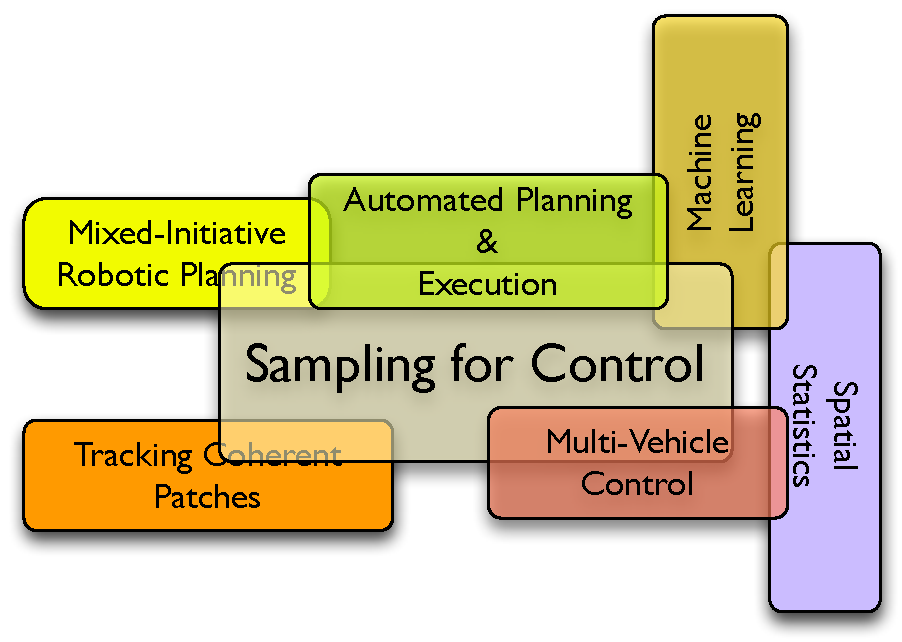
\includegraphics[scale=0.45]{figs/autonomy-topics.pdf}
  \caption{\small Overlapping topics in our research in deliberation
    and autonomy with sampling the dominant theme.}
  \label{fig:topics}
\end{figure}

The core of our problem domain for \can has been towards Sampling. In
large part given the spatial and temporal scales of the
bio-geochemical processes we are interested in, in this project, it is
imperative that a key direction is in formulating a multi-robot
adaptive sampling problem. In this context while \rx can be considered
as a 'multi-agent' system and \kcomment{could therefore imply its use
  in a multi-vehicle setting as} a direct extension, sporadic
communication with high-latencies in surface communication, not to
mention low throughput acoustic communications imply that the
extension of \rx for distributed applications is non-trivial. Further,
in order to efficiently execute coordinated observations of ocean
processes with multiple autonomous sensing platforms, significant
methodological as well as technical challenges must be
addressed. 

\kcomment{In this context} we are working towards a systematic
approach of using \rx as a backend planner \kcomment{within the \od}
for \can field experiments. The expectation is that \od users will
\kcomment{initially be able to} plan individual vehicle surveys which
\kcomment{would be} variants of straight-line transects. Lessons
learned with human planners in the loop will be used towards planning
larger surveys, also with simple fixed transects but using vehicle
capabilities in ontologies similar to \cite{patron09}. \kcomment{Doing
  so will likely enable the right vehicle to target an ocean feature
  with appropriate sensors and sampling strategy}. Apportioning the
planning task between shore-side components with substantial
contextual information and compute power, with robots having in-situ
reasoning capabilities similar to \rxe, is \kcomment{challenging in of
  itself} and an open research problem. \kcomment{In pursuing this
  line of research, we expect to touch on a range of associated
  problems for decision-theoretic control of vehicles in the coastal
  ocean}. Fig. \ref{fig:topics} shows what we believe is the scope and
influence of the different topic areas we are \kcomment{currently}
focusing on.

Partitioned inference and decision-making within \rx also lends itself
to graceful system degradation, making the overall approach effective
towards increased \kcomment{mission} robustness \kcomment{in the
  context of fault diagnosis, isolation and recovery (FDIR)}. There
are two outstanding diagnosis and failure recovery challenges that we
need to address; the first has to do with methodology related to model
design of the instrument payload for a highly modular and configurable
vehicle; this is local to a reactor. Doing so would enable (as a first
step) using systematic FDIR algorithms as demonstrated in the
\texttt{RAX} experiment \cite{williams96,mus98,williams97} and more
recently on AUVs \cite{wang09,ernits10,dearden11}. The second
challenge has to \kcomment{do with} implementing a policy within the
\rx framework that explicitly deals with recovery since controller
failure can be distributed across reactors. Since reactors are
hierarchical in their relationship to one another, their well defined
dependencies allow them to be removed from an agent systematically as
noted in Section \ref{sec:rx-reactor-failure}. Reactors more abstract
in scope can be removed before those which are less abstract (and
closer to the hardware). In the event a \texttt{Navigator} reactor,
for example, has a fault, it can be removed safely with lower level
functionalities (such as those in the executive). When the
\texttt{Navigator} is removed, it will recursively remove more
abstract reactors (such as a \texttt{Mission Manager}) that depend on
it. Such a safety feature then allows the system designers to ensure
that early on they can invest more in ensuring that reactors lower in
the hierarchy are robust and potentially formally verified. It also
means that there is a safe and sure way to take control of the vehicle
at any level within the reactors hierarchy; as long as low level
reactors are still active one will always been able to send
goals/commands to them and execute what are traditionally known as
runout sequences.

Feature recognition for Sampling is a general research thrust; however
it has specific relevance in the context of \rx and AUV control. As
noted in Section \ref{sec:results} we have already demonstrated
Machine Learning techniques for recognition of select features in the
coastal ocean. A principal challenge that remains is that of obtaining
expert labeled data for any supervised or semi-supervised learning
methods.  While supervised techniques for learning classifiers such as
decision trees (\cite{Quinlan93-dtrees}), instance-based
classification (\cite{Aha-ibl-ml91}), Bayesian classifiers
(\cite{Jensen2001-BNetworks}) and artificial neural networks
(\cite{ANNsurvey-2000}) are popular, given the vast amount of data
available and poor understanding of correlation between physical and
biogeochemical variables in the coastal ocean, our work on INLs
\cite{mcgann08d,ryan10} and reliance on a oceanographic expert has
shown that scaling to different problems remains problematic. This is
a prime motivation to move towards more semi-supervised methods such
as \cite{kumar11}. 

With the advent of the \od however, another direction our research is
taking us is in \texttt{Recommender Systems} \cite{Adomavicius05} as
noted in Section \ref{sec:results}. We are working to design and
deploy software infrastructure that will learn from user tagged
data. To do so, we will use tagging techniques similar to what users
of commercial image sharing sites like Flickr and Picassa do, to learn
the context of the data (including remote sensing). In addition, the
\od will integrate statistical Machine Learning techniques with
incoming asynchronous data stream obtained by sensors and
platforms. Identification models will be based on existing training
sets for INLs and plumes; models for other features of scientific
interests driven by \can requirements will be built in
addition. Existing AUV archives for instance provide sufficient data
for a learning base for a range of features of interest to scientists;
in addition we will build software that will learn to incorporate
incoming data streams to provide an existence proof of a feature of
interest.

A number of issues remain to be explored improving \rx and \eu
integration particularly in the context of engineering models for
execution.

Dispatchability of the {\em external} temporally flexible partial
plans continues to be an open research problem. Substantial progress
has been made \cite{vidal97,mus98a,tsam98,morris00} by analyzing the
plan structure of static offline temporal plans. However in the
context of embedded plan execution, balancing model design while
dealing with execution uncertainty requires further research. For
instance it should be possible to distinguish part of the plan that
contributes to a reactor goal, which often needs to be dispatched as
early as possible with other tokens describing world evolution with a
preference to dispatch as late as possible. Making this distinction
would improve the quality of agent behavior while avoiding extra model
complexity.

More abstractly at the architectural level, the ability to dynamically
manipulate the reactor graph would be of importance while creating new
reactors or modifying timelines. Doing so would provide more robust
failure recovery mechanisms especially after a reactor has failed to
synchronize. For example, an alternate reactor could take ownership of
timelines left invalid by the destruction of another failed reactor
ensuring a transparent implementation of component redundancy. While
the current design broadly provides for such a capability, the \rx API
has yet to implement it while ensuring other design elements within
are not compromised.

Finally and importantly, integration of reasoning about resources
within \rx and tying it to existing \eu capabilities needs to be
demonstrated. Specifically \rx needs to be able to update resource
levels as incoming observations.  Doing so would ensure plan
adaptation occurs dynamically when planned and observed resource
values diverge -- for instance if the vehicle looses a bank of
batteries during the course of a mission.  Enhanced modeling
capabilities and augmented domain-independent search within \eu would
make it easier for \rx users to create such domain models and to
perform more proactive deliberation.

Along with all these potential extensions, we are also very cognizant
that the learning curve associated with \rx and \eu for a general user
in the marine robotics community needs to be tackled. At present, the
complex system that underlies \rx and its underlying framework, even
if well documented, can be intimidating for a naive first time user.

% multi-vehicle control
% sampling
% diagnosis and recovery
% feature recognition
% scalable architecture for missions





%%% Local Variables: 
%%% mode: latex
%%% TeX-master: "setobook"
%%% End: 
